\subsection{Detailed Local Multiprocessing Study}
We extend the worker study to ten predefined workloads, three separate interpreter sessions on the same i7-13700H host, and one, two, or four worker processes. Each scientific runtime uses one thread. The operating system schedules processes across the allowed 20 logical CPUs; individual cores are not pinned, and this is not an isolated host. Within each workload, every policy executes the same experiment graph and reconstruction formulas, verified by a graph fingerprint. This isolates execution-policy effects from changes in plan quality.

Nine workloads contain independent components with seeded $R_Y$, $R_Z$, and nearest-neighbor CX layers. Widths range from four to 16 qubits, component counts from two to eight, and depths from four to 80 layers. A separate connected 16-qubit circuit joins two eight-qubit components with one CX and applies noncommuting terminal rotations; its exact cut plan contains 12 fragment tasks. Independent NumPy state-vector operations validate every collection. The reference is factorized only for the explicitly independent components and simulates all 16 qubits for the bridge case. This expands numerical coverage beyond the previous same-graph worker consistency check.

For each configuration, the first collection is recorded separately, followed by nine repetitions. Parent-side per-task diagnostic executions precede these collections, so ``first'' does not denote an uninitialized interpreter. Serial, forced parallel, and automatic-dispatch modes are interleaved in randomized order within a pool configuration; configuration and workload order vary across sessions. The study records 2,052 warm timed collections and 2,310 validated collections including first calls and separate resource probes. Maximum absolute error is $3.04\times10^{-15}$. Construction, cold planning, calibration, full pool warmup, shutdown, serialized recipe sizes, and execution phases are recorded separately. Detailed workload results are in Table~\ref{tab:local_parallel_full}.

\begin{figure*}[!t]
\centering
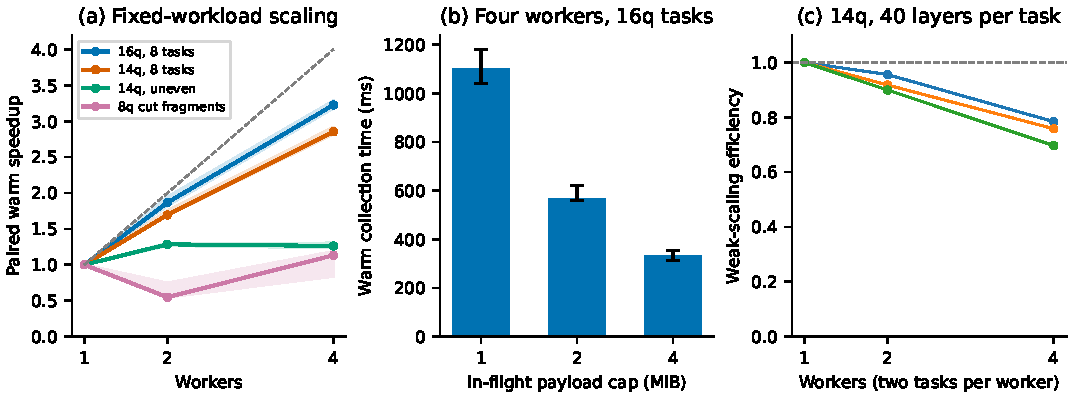
\includegraphics[width=\textwidth]{figures/local_parallel_scaling.pdf}
\caption{Measured local multiprocessing. (a) Fixed-workload speedups: lines show medians of three session-level paired geometric means; bands show their ranges, and the dashed line is ideal worker-count scaling. (b) Eight 16-qubit tasks on four workers under different aggregate payload caps: bars show medians of session medians, with session ranges. (c) Weak scaling holds two 14-qubit, 40-layer tasks per worker; each line is one session. All timings are warm and exclude setup.}
\label{fig:local_parallel_scaling}
\end{figure*}

\subsubsection{Strong Scaling and Task Granularity}
For each parallel policy, warm speedup is the geometric mean of paired serial/parallel time ratios; efficiency divides that speedup by the worker count. On eight 16-qubit components, four workers achieve $3.18\times$--$3.28\times$ speedup, corresponding to 79.6\%--82.1\% efficiency. Parallel median time is 313--355\,ms, while the separate one-worker configuration takes 1,028--1,169\,ms. The speedup uses paired serial controls within each pool configuration, so it need not equal the ratio of these independently summarized medians.

Eight balanced 14-qubit components reach $2.82\times$--$2.91\times$ on four workers. With only two components, four workers yield $1.68\times$--$1.71\times$: additional workers cannot create more independent tasks. An uneven eight-component batch, with seven four-layer components and one 80-layer component, yields only $1.24\times$--$1.30\times$. Its largest task limits completion time. Four-qubit components regress to $0.28\times$--$0.51\times$, while the connected bridge's cut fragments yield $0.84\times$--$1.19\times$. Thus the strongest scaling result concerns substantial independent tasks, not a demonstrated acceleration of connected-circuit cutting.

\subsubsection{Weak Scaling}
With two 14-qubit, 40-layer components per worker, the task count rises from two to eight as the worker count rises from one to four. Define weak-scaling efficiency as $T_1(2)/T_P(2P)$, using session median times. Four-worker efficiency is 69.7\%--78.4\%, and throughput grows from 29.7--32.4 to 90.0--93.5 tasks/s. The sublinear gain reflects the measured executor and shared host; it does not establish scaling beyond four processes.

\subsubsection{Setup Repayment and Time Allocation}
To assess short lifetimes, we sum the recorded first call and nine warm calls, adding construction, cold planning, and calibration once to both policies, plus full pool warmup and shutdown to parallel execution. This is cost accounting from interleaved observations, not a separately timed contiguous ten-call application. Full calibration takes 705--904\,ms per session; for the eight-task 16-qubit case, planning takes 210--343\,ms and four-worker warmup takes 103--146\,ms.

The 16-qubit workload retains a $2.56\times$--$2.63\times$ ten-call speedup with these charges, crossing break-even on the first recorded call in all three sessions. Eight balanced 14-qubit tasks retain $1.72\times$--$1.80\times$. In contrast, the shallow 14-qubit batch needs nine or ten calls to cross and ends at $1.00\times$--$1.02\times$; the ten-qubit batch remains slower despite its $1.19\times$--$1.25\times$ warm speedup. No later repayment is inferred for cases that do not cross within the observed horizon.

\begin{figure}[!t]
\centering
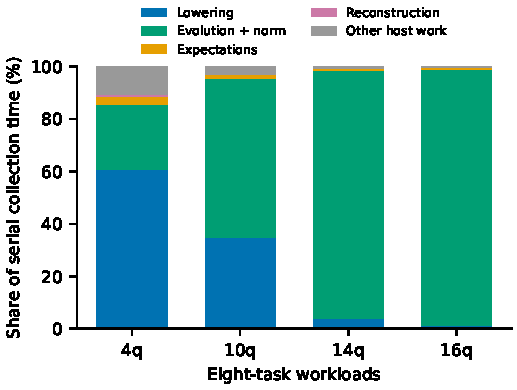
\includegraphics[width=\columnwidth]{figures/local_parallel_phases.pdf}
\caption{Time allocation in the one-worker configuration: mean per-call phase fractions over 27 warm observations per workload. Evolution includes initialization and norm checking. The residual includes host dispatch, cleanup, and instrumentation. These are serial wall-time fractions; parallel worker phase sums are not additive parent wall-time components.}
\label{fig:local_parallel_phases}
\end{figure}

Figure~\ref{fig:local_parallel_phases} explains the granularity dependence. Evolution and norm checking occupy approximately 25.0\% of serial collection time for the four-qubit workload, 60.9\% at ten qubits, 94.7\% at 14 qubits, and 98.0\% at 16 qubits. Native circuit lowering accounts for 60.8\% at four qubits. These workloads vary in depth as well as width, so the fractions characterize the tested configurations rather than a width-only law. Forced parallel execution avoids automatic-policy scoring, whose overhead remains visible: on the balanced eight-task 14-qubit workload, automatic dispatch achieves $2.58\times$--$2.62\times$, below forced parallelism.

\subsubsection{Memory, CPU, and Transport Costs}
For uniform independent tasks with payload $b$, worker count $P$, and aggregate payload budget $B$, at most $\min(P,\lfloor B/b\rfloor)$ tasks can be in flight, also bounded by available tasks. The 16-qubit states occupy 1\,MiB each. Holding four workers and the graph fixed, budgets of one, two, and four MiB yield speedups of $0.99\times$--$1.01\times$, $1.87\times$--$1.93\times$, and $3.18\times$--$3.28\times$, respectively (Fig.~\ref{fig:local_parallel_scaling}b). Provisioned processes alone do not supply usable parallelism when the payload budget serializes dispatch.

Resource measurements run in separate diagnostic collections to avoid sampling overhead in the timing trials. A 2\,ms target-period sampler reads Linux process RSS and CPU counters for the parent and the active pool. Summed sampled RSS counts shared pages once per process and may miss short peaks; it is neither unique physical memory nor an enforced RSS bound. CPU counters have 10\,ms resolution, so utilization ratios for probes shorter than 100\,ms are omitted.

For the eight-task 16-qubit workload, sampled parent-plus-pool RSS is 276--308\,MiB with four workers, compared with 147--174\,MiB serially, despite the much smaller four-MiB state-payload budget. Diagnostic CPU use is 1.29--1.38 CPU-s with four workers versus 1.04--1.14 CPU-s serially; lower latency does not imply less CPU work. The four-worker probes average approximately 3.85--4.01 CPU cores, including parent overhead. The four-worker pool still occupies roughly 276--308\,MiB when the payload cap is tightened, showing that payload throttling does not remove process overhead (Table~\ref{tab:local_parallel_resources}).

The eight 16-qubit task descriptions serialize to about 429\,KiB per collection before multiprocessing framing; results are scalar values and execution statistics. These are measured serialized object sizes, not monitored transport traffic. Numerical statevectors remain inside their executing process. The results therefore quantify a local multiprocessing trade-off among task granularity, available concurrency, setup repayment, and process footprint; they make no claim about networked or physical-QPU distribution.
